%%%%%%%%%%%%%%%%%%%%%%%%%%%%%%%%%%%%%%%%%%%%%%%%%%%%%%%%%%%%%%%%%%%%%%%%%%%%%%%%%%%%%%%%%%%%%%%%%%%%%%%%%%%%%%%%%%%%%%%%%%%%%%%%%%%%%%%%%%%%%%%%%%%%%%
%
\documentclass{amsart}
\newtheorem{lemma}{Lemma}
\usepackage{color,graphicx}
\title[Positive Forman curvature and corner curvature graphs]{
      Enumeration of simple, connected, planar, graphs with each corner having positive corner curvature, and     
      enumeration of simple, connected, planar graphs with each edge having positive Forman curvature~(Draft)
   }

%   \author{       Yohji Akama}%he visited Math. Dept., Fudan University on
%                                                                                                                     
%%%%%%%%%%%%%%%%%%%%%%%%%%%%%%%%%%%%%%%%%%%%%%%%%%%%%%%%%%%%%%%%%%%%%%%%%%%%%%%%%%%%%%%%%%%%%%%%%%%%%%%%%%%%%%%%%%%%%%%%%%%%%%%%%%%%%%%%%%%%%%%%%%%%%%


\date{\today} % 2019/12/4
\newtheorem{definition}{Definition}

\def\G{\mathcal{G}}
\def\PCnC{\mathcal{C\!\mathit{n}C}_{>0}}
\def\PFC{\mathcal{FC}_{>0}}
\usepackage{amsmath,tikz}
\begin{document}

\maketitle

\begin{abstract}
We enumerate all the 116 2-connected, simple, planar graphs such that
every edge has positive Forman curvature, by translating them into
4-regular graphs.  We enumerate all the 22 2-connected, simple, planar
graphs such that every corner has positive corner curvature.
\end{abstract}


\section{Introduction}
%%%%%%%%%%%%%%%%%%%%%%%%%%%%%%%%%%%%%%%%%%%%%%%%%%%%%%%%%%%%%%%%%%%%%%%%%%%%%%%%%%%%%%%%%%%%%%%%%%%%%%%%%%%%%%%%%%%%%%%%%%%%%%%%%%%%%%%%%%%%%%%%%%%%%%
 Let $\G$ be the set of connected, simple, planar 4-regular
graph $G=(V,E,F)$ such that  both of face degrees and vertex degrees are  at least
3 and finite.
For $G=(V,E,F)\in \G$  and an edge
$e\in E$, \emph{Forman-Ricci curvature} of $e$ is defined by:
\begin{align}
Ricc(e) =
16 - (|x_1|+|x_2|+|f_1|+|f_2|)  \label{def:ricci}
\end{align}
 where $e$ is $\{x_1, x_2\}$ and shared
by the two faces $f_1$ and $f_2$. Here $|x_i|$  is the degree of a
vertex $x_i$, and $|f_i|$ is the facial degree of a face
$f_i$. Forman-Ricci curvature of a graph is always an
integer and is defined for the edges. It is
 unlike combinatorial curvature.
 We are concerned with discrete
analogue of Bonnet-Myers theorem~\cite{MR2299456} for Forman-Ricci
curvature.
Let
\[
\PFC:=\{G\in \G\mid \mbox{$G$ has positive Forman-Ricci curvature everywhere}\}.
\]
If $G$ is in $\PFC$ then the dual $G^*$ is too. On the other hand, the
7-gonal prism $Prism_7$ has positive combinatorial curvature everywhere,
but the dual, the 7-gonal bipyramid, has negative curvature at the apexes.
We will prove that $\#\PFC<\infty$, by using
combinatorial curvature.
Then, we will enumerate them such $\PFC$.


To relate Forman-Ricci curvature with combinatorial curvature, we
translate a $G\in\G$ to a so-called \emph{meridian graph}, which is 4-regular.
\begin{definition}
By a \emph{meridian graph} of $G$, we mean   $m(G)=(V', E', F')\in\G$
 such that
 \begin{enumerate}
  \item  $V'=E$,

  \item  $\{e,e'\}\in E'\iff$ $e$ and $e'$ are
	 adjacent edges of a common face, and

  \item
	 $F'=F\cup V$ where (a) $\{e,e'\}\in E'$ is incident to $f\in
F$  in $m(G)$ $\iff$ $e$ and $e'$ are both incident to $f$ in $G$, (b) $\{e,e'\}\in
E'$ is incident to $v\in
 V$ in $m(G)$ $\iff$ $v$ is incident to $e$ and to $e'$ in $G$.
\end{enumerate}
\end{definition}
For example, the meridian graph of tetrahedron is the graph of the
octahedron, and the meridian graph of octahedron~(cube, resp.) is the
graph of the cuboctahedron, where the cuboctahedron is an Archimedean
solid.
An edge $e\in G$ is translated to a vertex of $m(G)$, and
the data $|x_i|$ and $|f_i|$ to define the Forman-Ricci curvature~\eqref{def:ricci} of an edge $e\in G$ is
translated as the environment of a vertex $e$ of $m(G)$.


We will first verify this translation is at most two-to-one.

\begin{lemma}
If $G'=(V',E',F')\in\G$ and $F'\ne\emptyset$, there is  $G\in\G$ such
 that $m(G)=G'$. $G$ is unique up to the duality.
\end{lemma}
     \begin{proof} Let $G'=(V',E',F')$. Take a $f_0\in F'$.
      \begin{itemize}
       \item
     Let $V$ be the
    least subset of $F'$ such that
    \begin{itemize}
     \item $f_0\in V$.
     \item If $f\in V$, $f'\in F'$, and there is a unique vertex $v\in
	   V'$ such that incident to
	   $f$ and to $f'$ in $G'$, then $f'\in V$.
    \end{itemize}

       \item
	     Let $F$ be $F'\setminus V$.

       \item Let $E$ be the set of
$\{f, f'\}\subseteq V$ such that $f\ne f'$ and there is a unique vertex
    $v\in V'$ incident to $f$ and to $f'$.

       \item Let $v\in V, \ e=\{f_1,f_2\}\in E,\ f \in F$. Then the
	     incidence relation $\prec_G$ of $G$ is defined as follows:
	     \begin{itemize}
	      \item $v\prec_G e:\iff v=f_1$ or $v=f_2$.
	      \item $v\prec_G f:\iff v$ is adjacent to $f$ in $G'$.
	      \item $e\prec_G f:\iff f_i$ is adjacent to $f$ $(i=1,2)$.
	     \end{itemize}
      \end{itemize}

      Because $G'$ is 4-regular and planar, for each $f\in F'$, (1) there is
      a unique $f'\in F'$ such that (*) there is only one $v'\in V'$ incident
      to $f$ and to $f'$, and (2) there are two $f'in F'$ such that
      $(*)$ does not hold. Hence, $V$ and $F$ are nonempty.

      We can prove that $m(G)=G'$.





 \end{proof}

Suppose a 4-degree vertex $v\in V$ of $G$ is shared by
 $p_1$-gon, $p_2$-gon, $p_3$-gon and $p_4$-gon where $p_1\le p_2\le
 p_3\le p_4$. Let us call $(p_1,p_2,p_3,p_4)$ the \emph{vertex pattern}
 of $v.$ Let us define
 \begin{align}
  \Phi(v)=16 - p_1 - p_2 - p_3 - p_4. \label{fc}
 \end{align}


Let $G=(V,E,F)$ be a connected, simple, planar 4-regular graph such that
both of face degrees and vertex degrees are at least 3, and $\Phi(v)>0$ for every
$v\in V$. Suppose $v\in V$ has
vertex pattern $(p_1, p_2, p_3, 7)$.
Then $p_1+p_2+p_3=5$ which is impossible because face degrees are at
least three. Hence, we have $p_4\le 6.$
%If $p_4=6$, then $p_i=3$ $(i=1,2,3)$, and thus $G$ is necessarily the 6-gonal antiprism.

 \begin{lemma} \label{lem:v}
  $m(\PFC):=\{m(G)\mid G\in\PFC\}$ is the \emph{finite} set of $G'\in\G$ such that
any vertex pattern is one of \begin{align}
(3,3,3,5),\ (3,3,3,4),\ (3,3,3,3),\ (3,3,4,4),\  (3,3,4,5),\
 (3,4,4,4),\ (3,3,3,6). \label{vp}
			     \end{align}
Moreover,   the number of vertices of $G'$ is greater than or equal to 6 and less
       than or equal to 24.
 \end{lemma}


  \begin{proof} By the definition of Forman-Ricci curvature and that of
   meridian graph, the vertex types are exactly as \eqref{vp}.

As to the finiteness, for any $G\in \PFC$,  observe that
the seven vertex types have combinatorial curvature greater than or
 equal to $1/12.$ The total combinatorial curvature is at most two
 by \cite{MR2299456}.
\end{proof}


We enumerate the finite set $m(\PFC)$ by a computer program. The program
is a modification of Brinkmann-MacKay's \texttt{plantri}.
\texttt{Plantri} can enumerates all of $\G$ such that the number of
vertices is at most 24. By modifying \texttt{plantri}, for all the
graphs $m(G)$ with the vertex patterns being one of \eqref{vp}, we
computed an inverse meridian graph $G$.


 As a result, we found that $m(\PFC)$ consists of 73 $m(G)$'s.  By
 examining an inverse meridian graph $G$ of the 73 $m(G)$'s, we found
 9 $G$'s are self-dual.  Hence, $\PFC$ consists of
 $30+(73-30)\times2=116$ tessellations.

  To describe the members of $\PFC$, we fix notations.
......






\begin{thebibliography}{1}

\bibitem{MR2299456}
M.~DeVos and B.~Mohar.
\newblock An analogue of the {D}escartes-{E}uler formula for infinite graphs
  and {H}iguchi's conjecture.
\newblock {\em Trans. Amer. Math. Soc.}, 359(7):3287--3300, 2007.
\bibitem{DS08} M.-M. Deza and  M. Dutour Sikir\'ic. Geometry of Chemical Graphs: Polycycles and Twofaced
Maps. Encyclopedia of Mathematics, Cambridge University Press, 2008.
\end{thebibliography}
\appendix
\section{All 116 2-connected, simple, planar graphs such that any edge
 has positive Forman curvature}

 Among the 116, there are one 6-edge self-dual graph, one 8-edge self-dual graph, 3
 10-edge self-dual graphs, 6 12-edge self-dual graphs, 4 14-edge
 self-dual graphs, 6 16-edge self-dual graphs, 4 18-edge self-dual
 graphs, 3 20-edge self-dual graphs, one 22-edge self-dual graph, and
 one 24-edge self dual graph.
 
  \def\a#1{\includegraphics[scale=0.2]{#1}}
 \begin{table}[ht]
     \begin{tabular}{|c|c|c|c || c|c|}
      \#E & \# & \#V & fig &\#V & the dual\\
\hline
 6 & 1 & 4 &  \\%&\includegraphics[scale=0.3]{E6_1V4Selfdual.fig}\\
 8 & 1 & 5 &  \\%E8_1V5Selfdual.fig
 9 & 1 & 6 &   &%E9_1V6.fig
         5 &  \\%E9_1V5Dual.fig
10 & 1 & 6 &  \\%E10_1V6Selfdual.fig
10 & 2 & 6 &  \\%E10_2V6Selfdual.fig
10 & 3 & 6 &  \\%E10_3V6Selfdual.fig
11 & 1 & 7 &   &%E11_1V7.fig
         6 &  \\%E11_1V6Dual.fig
11 & 2 & 7 &   &%E11_2V7.fig
         6 &  \\%E11_2V6Dual.fig
     \end{tabular}
\end{table}
\begin{table}[ht]
     \begin{tabular}{|c|c|c|c || c|c|}
      \#E & \# & \#V & fig & \#V &the dual\\
\hline
12 & 1 & 7 &  \\%E12_1V7Selfdual.fig
12 & 2 & 7 &  \\%E12_2V7Selfdual.fig
12 & 3 & 7 &  \\%E12_3V7Selfdual.fig
12 & 4 & 7 &  \\%E12_4V7Selfdual.fig
12 & 5 & 7 &  \\%E12_5V7Selfdual.fig
12 & 6 & 7 &  \\%E12_6V7Selfdual.fig
12 & 7 & 8 &  \\%E12_7V8.fig
         6 &  \\%E12_7V6Dual.fig
12 & 8 & 7 &   &%E12_8V7.fig
         7 &  \\%E12_8V7Dual.fig
12 & 9 & 7 &   &%E12_9V7.fig
         7 &  \\%E12_9V7Dual.fig
     \end{tabular}
\end{table}
\begin{table}[ht]
\begin{tabular}{|c|c|c|c || c|c|}
 \#E & \# & \#V & fig &\#V & the dual\\
 \hline
13 & 1 & 7 &   &%E13_1V7.fig
         8 &  \\%E13_1V8Dual.fig
13 & 2 & 7 &   &%E13_2V7.fig
         8 &  \\%E13_2V8Dual.fig
13 & 3 & 7 &   &%E13_3V7.fig
         8 &  \\%E13_3V8Dual.fig
13 & 4 & 8 &   &%E13_4V8.fig
         7 &  \\%E13_4V7Dual.fig
13 & 5 & 8 &   &%E13_5V8.fig
         7 &  \\%E13_5V7Dual.fig
13 & 6 & 7 &  &%E13_6V7.fig
         8 &  \\%E13_6V8Dual.fig
13 & 7 & 8 & &%E13_7V8.fig
         7 &   \\%E13_7V7Dual.fig
\end{tabular}
\end{table}
\begin{table}[ht]
\begin{tabular}{|c|c|c|c || c|c|}
      \#E & \# & \#V & fig &  \#V &the dual\\
\hline
14 & 10 & 8  &   \\%E14_10V8Selfdual.fig
14 & 1 & 8   && \\%E14_1V8Selfdual.fig
14 & 2 & 7   & &%E14_2V7.fig
         9   &   \\%E14_2V9Dual.fig
14 & 3 & 8   &  &%E14_3V8.fig
         8   &   \\%E14_3V8Dual.fig
14 & 4 & 8   &   \\%E14_4V8Selfdual.fig
14 & 5 & 8   &  &%E14_5V8.fig
         8   &   \\%E14_5V8Dual.fig
14 & 6 & 8   &   \\%E14_6V8Selfdual.fig
14 & 7 & 8   &  &%E14_7V8.fig
         8   &   \\%E14_7V8Dual.fig
14 & 8 & 8   &  &%E14_8V8.fig
         8   &   \\%E14_8V8Dual.fig
14 & 9 & 9   &  &%E14_9V9.fig
         7   &   \\%E14_9V7Dual.fig
\end{tabular}
\end{table}
\begin{table}[ht]
\begin{tabular}{|c|c|c|c || c|c|}
      \#E & \# & \#V & fig & \#V &the dual\\
\hline
15 & 1 & 8   &  &%E15_1V8.fig
         9   &   \\%E15_1V9Dual.fig
15 & 2 & 8   &  &%E15_2V8.fig
         9   &   \\%E15_2V9Dual.fig
15 & 3 & 9   &  &%E15_3V9.fig
         8   &   \\%E15_3V8Dual.fig
15 & 4 & 8   &  &%E15_4V8.fig
         9   &   \\%E15_4V9Dual.fig
15 & 5 & 8   &  &%E15_5V8.fig
         9   &   \\%E15_5V9Dual.fig
15 & 6 & 9   &  &%E15_6V9.fig
         8   &   \\%E15_6V8Dual.fig
15 & 7 & 9   &  &%E15_7V9.fig
         8   &   \\%E15_7V8Dual.fig
15 & 8 & 10  &   &%E15_8V10.fig
         7   &   \\%E15_8V7Dual.fig
\end{tabular}
\end{table}
\begin{table}[ht]
     \begin{tabular}{|c|c|c|c || c|c|}
\#E & \# & \#V & fig & \#V &the dual\\
      \hline
16 & 1 & 9   &   \\%E16_1V9Selfdual.fig
16 & 2 & 9   &  &%E16_2V9.fig
         9   &   \\%E16_2V9Dual.fig
16 & 3 & 9   &   \\%E16_3V9Selfdual.fig
16 & 4 & 9   &   \\%E16_4V9Selfdual.fig
16 & 5 & 9   &   \\%E16_5V9Selfdual.fig
16 & 6 & 9   &   \\%E16_6V9Selfdual.fig
16 & 7 & 9   &   \\%E16_7V9Selfdual.fig
16 & 8 & 10  &   &%E16_8V10.fig
         8   &   \\%E16_8V8Dual.fig
16 & 9 & 8   &  &%E16_9V8.fig
         10  &    \\%E16_9V10Dual.fig
\end{tabular}
\end{table}
\begin{table}[ht]
     \begin{tabular}{|c|c|c|c || c|c|}
      \#E & \# & \#V & fig & \#V &the dual\\
\hline
17 & 1 & 10  &   &%E17_1V10.fig
         9   &   \\%E17_1V9Dual.fig
17 & 2 & 10  &   &%E17_2V10.fig
         9   &   \\%E17_2V9Dual.fig
17 & 3 & 9   &  &%E17_3V9.fig
         10  &    \\%E17_3V10Dual.fig
17 & 4 & 9   &  &%E17_4V9.fig
         10  &    \\%E17_4V10Dual.fig
\end{tabular}
\end{table}
\begin{table}[ht]
     \begin{tabular}{|c|c|c|c || c|c|}
      \#E & \# & \#V & fig &  \#V &the dual\\
\hline
18 & 1 & 10  &    \\%E18_1V10Selfdual.fig
18 & 2 & 10  &    \\%E18_2V10Selfdual.fig
18 & 3 & 10  &   &%E18_3V10.fig
         10  &    \\%E18_3V10Dual.fig
18 & 4 & 9   &  &%E18_4V9.fig
         11  &    \\%E18_4V11Dual.fig
18 & 5 & 10  &    \\%E18_5V10Selfdual.fig
18 & 6 & 10  &    \\%E18_6V10Selfdual.fig
18 & 7 & 9   &  &%E18_7V9.fig
         11  &    \\%E18_7V11Dual.fig
18 & 8 & 10  &   &%E18_8V10.fig
         10  &    \\%E18_8V10Dual.fig
\end{tabular}
\end{table}
\begin{table}[ht]
     \begin{tabular}{|c|c|c|c || c|c|}
      \#E & \# & \#V & fig & \#V &the dual\\
\hline
19 & 1 & 11  &   &%E19_1V11.fig
         10  &    \\%E19_1V10Dual.fig
19 & 2 & 10  &   &%E19_2V10.fig
         11  &    \\%E19_2V11Dual.fig
19 & 3 & 10  &   &%E19_3V10.fig
         11  &    \\%E19_3V11Dual.fig
20 & 1 & 11  &    \\%E20_1V11Selfdual.fig
20 & 2 & 11  &    \\%E20_2V11Selfdual.fig
20 & 3 & 11  &    \\%E20_3V11Selfdual.fig
\end{tabular}
\end{table}
\begin{table}[ht]
     \begin{tabular}{|c|c|c|c || c|c|}
      \#E & \# & \#V & fig & \#V &the dual\\
\hline
21 & 1 & 12  &   &%E21_1V12.fig
         11  &    \\%E21_1V11Dual.fig
22 & 1 & 12 &   \\%E22_1V12Selfdual.fig
24 & 1 & 14 &    &%E24_1V14.fig
         12 &       \\%E24_1V12Dual.fig
24 & 2 & 13  &    \\%E24_2V13Selfdual.fig
     \end{tabular}
\end{table}
\section{All 22 2-connected, simple, planar graphs such that any edge has positive corner
 curvature}
 Among the 22, there are one 4-edge self-dual graph, one 8-edge self-dual graph, one
9-edge self-dual graphs, and
 one 10-edge self dual graph. See Table~\ref{tbl:PCnC} for Schlegel
 diagrams or 3d representations of the 22 graphs.

 
\begin{table}[ht]
     \begin{tabular}{|c|c|c|c || c|c|c|}
      \#E & \# & \#V & graph  &  \#V &the
      dual  & PFC?\\
\hline
\hline
4 & 1 & 4  & Regular tetrahedron  &4&Regular tetrahedron &YES\\ %#1/13
\hline
8 & 1 & 5  & Square pyramid &5& Square pyramid &YES \\ %#3/13
\hline
9 & 1 & 5  & Triangular bipyramid &5& Triangular bipyramid &YES \\ %#2/13
\hline
10 & 1 & 6  & Pentagonal pyramid  &6& Pentagonal pyramid &YES  \\ %#5/13
\hline
      12 & 1 & 6  & \begin{tabular}{c}
	       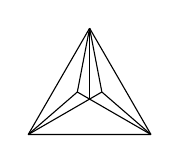
\begin{tikzpicture}[scale=.5]
\begin{scope}[scale=0.9]
\foreach \x in {1,...,3}
{
\draw[rotate=120*\x]
  (90:2) -- (210:2);
\draw[rotate=120*\x]
  (90:2) -- (0:0);

 }
\draw (90:2) -- (150:0.4) -- (210:2);  
  \draw (0:0) -- (150:0.4);
\begin{scope}[xscale=-1]
 \draw (90:2) -- (150:0.4) -- (210:2);  
\draw (0:0) -- (150:0.4);  x
\end{scope}
	       \end{scope}\end{tikzpicture}\\
		    Biaugmented tetrahedron\end{tabular}
  &
 8  & \begin{tabular}{c}
       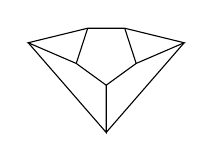
\begin{tikzpicture}[scale=.5]
       \begin{scope}[rotate=90,xscale=-1]

\foreach \x in {1,...,5}
{
\draw[rotate=72*\x]
	(0:0.8) -- (72:0.8);
}

 \draw (0:.8) --(0:2) -- (98:2);
 \draw (262:2) -- (0:2);
 \draw (216:.8) --(262:2) -- (288:.8);
 \draw (72:.8) --(98:2) -- (144:.8);
\end{scope}     \end{tikzpicture}      \end{tabular}  &NO \\ %#4/13
\hline
12 & 1 & 6  & Regular octahedron & 8  & Cube  &YES \\ %#6/13
\hline
15 & 1 & 7  & Pentagonal bipyramid & 10 & Pentagonal prism  &YES\\ %#7/13
\hline
15 & 2 & 7  &\begin{tabular}{c}	       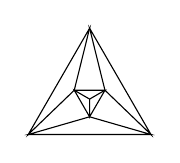
\begin{tikzpicture}[scale=0.5]
\begin{scope}[scale=0.9]
\foreach \x in {1,...,3}
{
\draw[rotate=120*\x]
  (90:2) -- (210:2)--(150:0.5)--cycle;
\draw[rotate=120*\x]
  (0:0) --  (150:0.5) -- (270:0.5);
 }
\end{scope}
\end{tikzpicture} 
     \end{tabular} &
 10  & \begin{tabular}{c}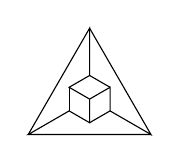
\begin{tikzpicture}[scale=0.5]
  
\begin{scope}[scale=0.6,xshift=10cm]
\foreach \x in {0,...,2}
{
\draw[rotate=120*\x]  (210:3)--(90:3) -- (90:1) -- (150:1)--(0:0);
 \draw[rotate=120*\x] (210:1)--(150:1);
}
\end{scope}
 \end{tikzpicture}\end{tabular}&NO\\
\hline
18 & 1 & 8  & \begin{tabular}{c}
	       \includegraphics[scale=0.3]{GyroelongatedTriangularBipyramid.pdf} \\
	       Gyroelongated triangular\\
	       bipyramid\\
	       \end{tabular} &
12  & $\begin{array}{c} 
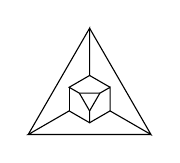
\begin{tikzpicture}[scale=.5]
		\begin{scope}[scale=0.6,xshift=10cm]
\foreach \x in {0,...,2}
{
\draw[rotate=120*\x]  (210:3)--(90:3) -- (90:1) -- (150:1)--(150:.5)--(30:.5);
 \draw[rotate=120*\x] (210:1)--(150:1);
}
\end{scope}
\end{tikzpicture}\\
\mbox{Snub $Prism_3$ \cite[p.20]{DS08}}
       \end{array}$
 &NO \\ %#9/13
\hline
18 & 2 & 8  & $\begin{array}{c}
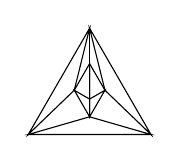
\begin{tikzpicture}[scale=0.5]
\begin{scope}[scale=0.9]
\foreach \x in {1,...,3}
{
\draw[rotate=120*\x]
  (90:2) -- (210:2)--(150:0.5)--cycle;
}

 \draw  (0:0) --  (150:0.5) -- (270:0.5)--(90:1);
 \draw  (0:0) --  (30:0.5) -- (270:0.5)--(90:1);

 \draw (30:.5) -- (90:1) -- (150:.5);
 \draw (90:2) -- (90:1);
\end{scope}
\end{tikzpicture} \\
		\mbox{Snub disphenoid~($J_{84}$)}
	       \end{array}$
&
 12  & \begin{tabular}{c}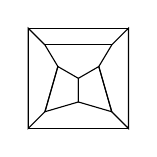
\begin{tikzpicture}[scale=0.5]  
\begin{scope}[scale=0.6,xshift=10cm]
\draw  (135:3)--(135:2) -- (150:1) -- (225:2)--(225:3)--cycle;
 \draw (0:0)--(150:1)--(225:2)--(270:1)--cycle;
 \draw (45:2)--(135:2);
 \draw (45:3)--(135:3);
 \draw (225:3)--(315:3);  
\end{scope}
\begin{scope}[scale=0.6,xshift=10cm,xscale=-1]
\draw  (135:3)--(135:2) -- (150:1) -- (225:2)--(225:3)--cycle;
 \draw (0:0)--(150:1)--(225:2)--(270:1)--cycle;
 \draw (45:2)--(135:2);
 \draw (45:3)--(135:3);
 \draw (225:3)--(315:3);  
\end{scope}
	       \end{tikzpicture}\end{tabular}  &NO \\ %#10/13
\hline
21 & 1 & 9  & \begin{tabular}{c}
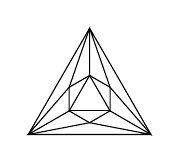
\begin{tikzpicture}[scale=0.5]
	       \begin{scope}[scale=0.6,yshift=1.5cm]
\foreach \x in {0,...,2}
{
\draw[rotate=120*\x]  (210:3)--(90:3) -- (90:1) -- (150:1)--cycle;
 \draw[rotate=120*\x] (210:1)--(150:1)--(90:3);
  \draw[rotate=120*\x] (-150:1)--(90:1);
}
\end{scope}
	      \end{tikzpicture} \\ Triaugmented triangular prism ($J_{51}$)\end{tabular}		    &
13  & 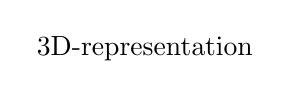
\begin{tikzpicture}[scale=.5]
		\begin{scope}[scale=0.6,xshift=10cm]
 \node at (0,2) {3D-representation};
\end{scope}
      \end{tikzpicture}&NO   \\ %#11/13
\hline
24 & 1 & 10 & \begin{tabular}{l}
	       (3d) representation \\
	       \\
	       Gyroelongated square\\
	       bipyramid ($J_{17}$)\\
	       \end{tabular}&
 16 &  $\begin{array}{c}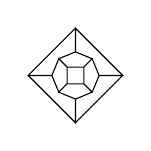
\begin{tikzpicture}[scale=.5]
		  
\begin{scope}[scale=0.6,xshift=10cm,yshift=1.5cm,yscale=-1]
\foreach \x in {0,...,3}
{
\draw[rotate=90*\x]  (180:2)--(90:2) -- (90:1) -- (135:1)--(135:.5)--(45:.5);
 \draw[rotate=90*\x] (180:1)--(135:1);
}
\end{scope}
      \end{tikzpicture}\\ \mbox{Snub $Prism_4$ \cite[p.20]{DS08}}\end{array}$&NO\\  %#12/13
\hline
30 & 1 & 12 & Regular icosahedron      &
		      20 & Regular dodecahedron &NO     \\  %#13/13
      \hline
     \end{tabular}
 \caption{All the 22 2-connected, simple, planar graphs such that every corner
 curvature is positive. \label{tbl:PCnC}}
\end{table}
 
\end{document}

\appendix
\section{All 73 simple, 2-connected, meridian graphs}
  \def\a#1{\includegraphics[scale=0.2]{#1}}
 \begin{figure}[ht]
    \begin{tabular}{ccc}
\a{MeridianImage/4_1.pdf}&
     \a{MeridianImage/5_2.pdf}\\
     \a{MeridianImage/6_4.pdf}&
\a{MeridianImage/6_3.pdf}&
\a{MeridianImage/6_5.pdf}\\
\a{MeridianImage/6_6.pdf}&
    \end{tabular}
  \caption{One 4-vertex graph, one 5-vertex graph, four 6-vertex graph.
  The first three and the last two are self-dual.}
   \end{figure}
 \begin{figure}[ht]
     \begin{tabular}{ccc}
      \a{MeridianImage/7_14.pdf}&
      \a{MeridianImage/7_9.pdf} &
      \a{MeridianImage/7_10.pdf}\\
\a{MeridianImage/7_11.pdf}&
\a{MeridianImage/7_12.pdf}&
\a{MeridianImage/7_13.pdf}\\
\a{MeridianImage/7_16.pdf}&
\a{MeridianImage/7_17.pdf}&
\a{MeridianImage/7_18.pdf}\\
\end{tabular}
  \caption{15 7-vertex graphs~(continued). The first two and the fifth are self-dual.}
 \end{figure}
 \begin{figure}[ht]
    \begin{tabular}{ccc}
\a{MeridianImage/7_20.pdf}&
\a{MeridianImage/7_23.pdf}&
\a{MeridianImage/7_26.pdf}\\
\a{MeridianImage/7_7.pdf}&
	 \a{MeridianImage/7_8.pdf}&
	      \a{MeridianImage/7_19.pdf}\\
\\
     \end{tabular}
  \caption{15 7-vertex graphs. }
 \end{figure}
 \begin{figure}[ht]
    \begin{tabular}{ccc}
\a{MeridianImage/8_15.pdf}&
\a{MeridianImage/8_21.pdf}&
\a{MeridianImage/8_22.pdf}\\
\a{MeridianImage/8_24.pdf}&
\a{MeridianImage/8_25.pdf}&
\a{MeridianImage/8_27.pdf}\\
\a{MeridianImage/8_28.pdf}&
\a{MeridianImage/8_29.pdf}&
\a{MeridianImage/8_30.pdf}
    \end{tabular}
  \caption{17 8-vertex graphs~(continued).}
  \end{figure}
   \begin{figure}[ht]
    \begin{tabular}{ccc}
\a{MeridianImage/8_31.pdf}&
\a{MeridianImage/8_32.pdf}&
\a{MeridianImage/8_34.pdf}\\
\a{MeridianImage/8_35.pdf}&
\a{MeridianImage/8_36.pdf}&
\a{MeridianImage/8_38.pdf}\\
\a{MeridianImage/8_39.pdf}&
  \a{MeridianImage/8_51.pdf}&
 \end{tabular}
  \caption{17 8-vertex graphs.}
   \end{figure}
 \begin{figure}[ht]
  \begin{tabular}{ccc}
   \a{MeridianImage/9_33.pdf}&
   \a{MeridianImage/9_37.pdf}&
   \a{MeridianImage/9_40.pdf}\\
   \a{MeridianImage/9_41.pdf}&
   \a{MeridianImage/9_43.pdf}&
   \a{MeridianImage/9_44.pdf}\\
   \a{MeridianImage/9_45.pdf}&
   \a{MeridianImage/9_46.pdf}&
   \a{MeridianImage/9_47.pdf}
  \end{tabular}
  \caption{15 9-vertex graphs~(continued). The second is self-dual.}
\end{figure}
 \begin{figure}[ht]
    \begin{tabular}{ccc}
\a{MeridianImage/9_48.pdf}&
\a{MeridianImage/9_49.pdf}&
\a{MeridianImage/9_54.pdf}\\
\a{MeridianImage/9_55.pdf}&
\a{MeridianImage/9_62.pdf}&
\a{MeridianImage/9_59.pdf}
     \end{tabular}
  \caption{15 9-vertex graphs.}
 \end{figure}
 \begin{figure}[ht]
  \begin{tabular}{ccccc}
\a{MeridianImage/10_42.pdf}&
\a{MeridianImage/10_50.pdf}&
\a{MeridianImage/10_52.pdf}\\
\a{MeridianImage/10_53.pdf}&
\a{MeridianImage/10_56.pdf}&
\a{MeridianImage/10_57.pdf}\\
\a{MeridianImage/10_58.pdf}&
\a{MeridianImage/10_60.pdf}&
  \a{MeridianImage/10_61.pdf}\end{tabular}
  \caption{12 10-vertex graphs~(continued).}
 \end{figure}
 \begin{figure}[ht]
    \begin{tabular}{ccc}
 \a{MeridianImage/10_63.pdf}&
\a{MeridianImage/10_65.pdf}&
\a{MeridianImage/10_66.pdf}
  \end{tabular}
  \caption{12 10-vertex graphs.}
 \end{figure}
 \begin{figure}[ht]
    \begin{tabular}{ccc}
\a{MeridianImage/11_64.pdf}&
\a{MeridianImage/11_67.pdf}&
\a{MeridianImage/11_68.pdf}\\
     \a{MeridianImage/11_69.pdf}&&
	 \end{tabular}
  \caption{Four 11-vertex graphs. The third is self-dual.}
 \end{figure}
 \begin{figure}[ht]
    \begin{tabular}{ccc}
\a{MeridianImage/12_70.pdf}&
     \a{MeridianImage/12_71.pdf}&
     \a{MeridianImage/12_72.pdf}\\
     \a{MeridianImage/13_73.pdf}&&\\
%     \a{MeridianImage/14_72.pdf}&&\\
    \end{tabular}
  \caption{Three 12-vertex graphs, one 13-vertex graph.}
   \end{figure}

\end{document}
\section{Operations for $m(\PFC)$}

  it
is convenient to introduce a \emph{pinching} of a simple, planar graph.
       Suppose that a simple, planar graph $G$ has a square face $(v_1,v_2,v_3,v_4)$.
 We say $G'$ is a \emph{pinched} $G$, if $G'=G\setminus\{(v_1,v_2),\
       (v_3,v_4)\} + \{ (v_i, u)\ \mid\ i=1,2,3,4\}$ where $u$ is a new
       vertex.
       In this case, we say $G$ is \emph{released} $G'$.

The graphs of $\PFC$ are  generated from the following graphs by means of finite
applications of the following local operations of $\PFC$.
\begin{itemize}
 \item $r$-gonal antiprism $AP_r$ ($r=4,5,6$)

 \item  Regular octahedron~(=$3$-gonal antiprism),

 \item One  Archimedean solid:

       Cuboctahedron,

\end{itemize}
\begin{itemize}


 \item 9 Johnson solids:
\begin{itemize}
 \item  $J_7,\ J_8,\ J_9$ are elongated
       $r$-gonal prisms $(r=3,4,5)$
 \item
       Elongated square bipyramid (=$J_{15}$),
 \item Triangular
	     orthobicupola~$(=J_{27})$,
 \item Square orthobicupola~$(=J_{28})$,
 \item Square	     gyrobicupola~$(=J_{29})$,
 \item Elongated triangular		   orthobicupola~$(=J_{35})$,
 \item Elongated triangular		 gyrobicupola~$(=J_{36})$,
 \item Elongated square gyrobicupola~$(=J_{37})$,
\end{itemize}

 \item $m(Prism_r)$ $(r=3,4,5)$ where $Prism_r$ is the $r$-gonal prism.




%It is obtained as follows: First consider an $r$-gon. Surround it by      $r$ 3-gons. Then surround it by $r$ 4-gons, twice.
%Finally, for the $r$ outermost vertices, join adjacent outermost  vertices to have additional $r$ 3-gons and the outer plane $r$-gon.

       Note that
       \begin{itemize}
	\item $m(Pyramid_r)=AP_r$. Here $Pyramid_r$ is the $r$-gonal pyramid and
	      $AP_r$ is the $r$-gonal antiprism.

	      The vertices are  $u_i, v_{i}$ $(i=0,\ldots,r-1)$, the
	      edges are $\{u_i,u_{i+1\bmod r}\}$,  $\{v_i,v_{i+1\bmod
	      r}\}$, and $\{u_i,v_i\}$ $(i=0,\ldots,r-1)$.
	      The facial walks are $u_0u_1\cdots u_{r-1}$,
	      $v_0v_1\cdots v_{r-1}$, $u_i u_{i+1\bmod r} v_{i+1\bmod r}
	      v_i$ $(i=0,\ldots,r-1)$.

	\item $m(AP_4)=J_{29}$.
	\item $m(m(Prism_3))=J_{35}$.
	\item $m(Prism_4)=m(Octahedron)$ is cuboctahedron, and the $m(Prism_r)$ is the simultaneous pinch of $r$-gonal prism.
       \end{itemize}


%       The vertices are $u_i,v_i,w_i$ $(i=1,\ldots,r)$.
%      The edges are  $(u_i,u_{i+1\bmod r}),\ (v_i,v_{i+1\bmod r})$,
%      $(u_i, w_i),\ (v_i,w_i), \ (u_{i+1\bmod r}, w_i), \ (v_{i+1\bmod
       %      r}, w_i).$
%       The faces are $2r$ 3-gons $(u_i,u_{i+1\bmod r},  w_i),\ (v_i,v_{i+1\bmod r}, w_i)$, $r$ 4-gons $(u_i,w_{i-1\bmod       r}, v_i, w_i)$, and  two $r$-gons $(u_1,u_2,\ldots,u_r),\       (u_1,u_2,\ldots,u_r)$.
\end{itemize}
The local operations are:
\begin{itemize}
 \item Flipping

Suppose that in $G\in\PFC$ there are vertices
       $u,v,u_i,v_i$ $(i=1,2,3)$ and the following nine edges
\begin{align*}
(u, v),\quad
( u, u_i), \ ( v, v_i)\ (i=1,2,3),\quad
( u_3, v_1),\ ( v_3, u_1)
\end{align*}
such that
\begin{itemize}
 \item  $(u,v,v_3,u_1)$ and $(v,u,u_3,v_1)$ are faces of $G$,
 \item For $j=1,2$, there is a face $f$ of $G$, such that  $(u,u_j)$ and
       $(u,u_{j+1})$ are adjacent edges of $f$.
 \item For $j=1,2$, there is a face $f$ of $G$, such that  $(v,v_j)$ and $(v,v_{j+1})$ are adjacent edges of $f$.

\end{itemize}
       We say $G'\in \PFC$ is a \emph{flipped~($F$ for short)} $G$, if $G'=G\setminus\{(u, u_3),\
       (v,v_3)\} +\{(u,v_1),\ (v,u_1)\}$. In

 \item Pinching
 \item Pinching after Divorce~(PD for short)

       See Figure~\ref{fig:pd}
       \begin{figure}[h]
	%	\includegraphics[scale=0.4]{.}
%	\includegraphics[scale=0.4]{.}
	%		\includegraphics[scale=0.4]{.}
	\caption{(a) Original (b) Divorce~(middle) (c) Pinching after divorce~(right).\label{fig:pd}}
       \end{figure}
\end{itemize}

\end{document}

The first line is the number of vertex of type 3335,
 		   the number of vertex of type 3334,  the number of
		   vertex of type 3333,  the number of vertex of type
		   3344,  the number of vertex of type 3345,  the number
		   of vertex of type 3444, and then the number of
		   vertices, the number of 3-gons, the number of 4-gons,
		   and the number of 5-gons.

		   The second line is the adjacent list.  The vertices of
     the graph are named by ASCII characters starting with 'a'.  The
     first word is the neighbors of 'a' in clockwise order, the second
     word is those of 'b' in clockwise order, and so  on.

\begin{enumerate}
 \item Octahedron

0	0	6	0	0	0	|	6	8
       0	0


$ bcde,aefc,abfd,acfe,adfb,bedc$
 \item  4-gonal Antiprism

0	8	0	0	0	0	|	8	8	2	0

$ bcde,aefg,aghd,ache,adfb,behg,bfhc,cgfd$
 \item
0	6	0	3	0	0	|	9	8	3	0

$ bcde,aefg,aghd,acie,adib,bihg,bfhc,cgfi,dhfe$

 \item 5-gonal Antiprism
10	0	0	0	0	0	|	10	10	0	2

$ bcde,aefg,ahid,acie,adfb,bejg,bfjh,cgji,chjd,fihg$
 \item
0	4	0	6	0	0	|	10	8	4	0

$ bcde,afgh,ahid,acje,adjf,bejg,bfih,bgic,chgj,dife$
 \item
0	0	2	8	0	0	|	10	8	4	0

$ bcde,afgh,ahid,acie,adif,bejg,bfjh,bgjc,cjed,fihg$
 \item
3	3	0	2	2	1	|	11	9	3	1

$ bcde,aefg,ahid,acij,ajfb,bekg,bfkh,cgki,chjd,dike,fjhg$
 \item
0	2	0	9	0	0	|	11	8	5	0

$ bcde,aefg,aghd,acij,ajkb,bkhg,bfhc,cgfi,dhkj,dike,ejif$
 \item
4	2	0	0	6	0	|	12	10	2	2

$ bcde,aefg,ahij,ajke,adfb,belg,bflh,cgli,chkj,cikd,djil,fkhg$
 \item
0	2	0	8	0	2	|	12	8	6	0

$ bcde,aefc,abgh,ahij,ajfb,bekg,cfkl,clid,dhlj,dike,fjlg,gkih$
 \item
0	6	0	0	0	6	|	12	8	6	0

$ bcde,afgh,ahid,acij,ajkf,bekg,bfkl,blic,chjd,dile,elgf,gkjh$
 \item
0	4	0	4	0	4	|	12	8	6	0

$ bcde,aefc,abgd,acgh,ahib,bijg,cfkd,dkle,eljf,filk,gjlh,hkji$
 \item
0	0	0	12	0	0	|	12	8	6	0

$ bcde,aefg,aghi,aije,adkb,bklg,bfhc,cgli,chjd,dilk,ejlf,fkjh$
 \item
0	0	0	12	0	0	|	12	8	6	0

$ bcde,aefg,aghd,acij,ajkb,bklg,bfhc,cgli,dhlj,dike,ejlf,fkih$
 \item
2	2	0	4	3	1	|	12	9	4	1

$ bcde,aefg,ahid,acij,ajfb,bekg,bfkh,cgli,chld,dlke,fjlg,hkji$
 \item
1	2	1	2	4	2	|	12	9	4	1

$ bcde,aefg,ahij,ajke,adfb,bekg,bfkh,cgli,chlj,cild,dlgf,hkji$
 \item
3	1	0	2	7	0	|	13	10	3	2

$ bcde,aefg,ahij,ajke,adfb,belg,bflh,cgmi,chmj,cikd,djml,fkmg,hlki$
 \item
0	0	0	11	0	2	|	13	8	7	0

$ bcde,afgc,abhi,aije,adkf,bekg,bflh,cglm,cmjd,dimk,ejlf,gkmh,hlji$
 \item
1	2	0	4	4	2	|	13	9	5	1

$ bcde,aefc,abgh,ahie,adjb,bjkl,clmh,cgmd,dmkj,eikf,fjil,fkmg,glih$
 \item
2	0	0	7	3	1	|	13	9	5	1

$ bcde,aefg,aghi,aije,adjb,bklg,bflc,clmi,chmd,dmke,fjml,fkhg,hkji$
 \item
0	2	1	0	10	0	|	13	10	3	2

$ bcde,aefc,abgd,achi,aijb,bklg,cflm,dmji,dhje,eihk,fjml,fkmg,glkh$
 \item
0	2	0	7	0	4	|	13	8	7	0

$ bcde,afgc,abhi,aije,adjf,bekg,bflh,cglm,cmjd,dike,fjml,gkmh,hlki$
 \item
1	2	0	4	4	2	|	13	9	5	1

$ bcde,aefc,abgh,ahie,adib,bjkg,cfkl,clmd,dmje,fimk,fjlg,gkmh,hlji$
 \item
2	0	0	4	8	0	|	14	10	4	2

$ bcde,aefg,ahij,ajke,adfb,belg,bfmh,cgmi,chnj,cikd,djnl,fknm,glnh,imlk$
 \item
1	0	0	7	4	2	|	14	9	6	1

$ bcde,afgc,abhi,aije,adkf,bekg,bflm,cmni,chnd,dnlk,ejlf,gkjm,glnh,hmji$
 \item
0	1	0	8	0	5	|	14	8	8	0

$ bcde,aefc,abgh,ahij,ajkb,bklg,cflm,cmid,dhnj,dike,ejnf,fnmg,glnh,imlk$
 \item
0	2	0	6	0	6	|	14	8	8	0

$ bcde,aefc,abgh,ahij,ajfb,bekg,cflm,cmid,dhnj,dike,fjnl,gknm,glnh,imlk$
 \item
1	0	0	7	4	2	|	14	9	6	1

$ bcde,aefg,aghd,acij,ajfb,bekl,blhc,cgmi,dhnj,dine,fnml,fkmg,hlkn,imkj$
 \item
0	2	0	6	0	6	|	14	8	8	0

$ bcde,afgc,abgd,achi,aijf,bejk,bkhc,dgli,dhme,emnf,fnlg,hknm,ilnj,jmlk$
 \item
0	0	0	10	0	4	|	14	8	8	0

$ bcde,aefg,aghi,aije,adkb,bklg,bflc,clmi,chmd,dmnk,ejnf,fnhg,hnji,jmlk$
 \item
0	2	0	4	5	3	|	14	9	6	1


$ bcde,aefg,ahij,ajke,adlb,blmg,bfmh,cgni,chnj,cikd,djnl,ekmf,flng,hmki$
 \item
0	2	0	2	10	0	|	14	10       4	2


$ bcde,aefg,ahij,ajke,adkb,bklg,bfmh,cgmi,chnj,cind,dlfe,fknm,glnh,imlj$
 \item
0	0	0	10	0	4	|	14	8	8	0

$ bcde,afgc,abhi,aije,adjf,bekg,bflh,cglm,cmnd,dnke,fjnl,gkmh,hlni,imkj$
\item
0	0	0	9	0	6	|	15	8	9	0

$ bcde,afgc,abgh,ahie,adjf,bejk,bklc,clmd,dmnj,einf,fnog,gomh,hloi,iokj,knml$
 \item
0	1	0	7	0	7	|	15	8	9	0

$   bcde,afgc,abhi,aije,adkf,bekg,bflh,cgmn,cnod,dolk,ejlf,gkjm,hlon,hmoi,inmj$
 \item
0	1	0	7	0	7	|	15	8	9	0

$       bcde,aefg,aghd,acij,ajfb,bekl,blhc,cgmi,dhnj,dike,fjno,fomg,hlon,imok,knml$
 \item
1	0	0	4	9	1	|	15	10	5	2

$      bcde,afgc,abhd,acij,ajkf,bekg,bflh,cglm,dmnj,dine,enof,gomh,hloi,iokj,knml$
 \item
1	0	0	6	4	4	|	15	9	7	1

$
       bcde,afgc,abhd,achi,aijf,bekg,bflm,cmnd,dnje,eiok,fjol,gkom,glnh,hmoi,jnlk$
 \item
0	1	0	5	5	4	|	15	9	7	1

$       bcde,aefg,aghi,aije,adkb,blmg,bfhc,cgmi,chnd,dnok,ejol,fkom,flnh,imoj,jnlk$
 \item
0	0	0	7	5	3	|	15	9	7	1

$
       bcde,aefc,abgh,ahij,ajkb,blmg,cfmh,cgnd,dnoj,dike,ejol,fkom,flng,hmoi,inlk$
 \item
0	0	0	5	10	0	|	15	10	5	2

$
       bcde,aefg,ahid,acjk,aklb,blmg,bfnh,cgni,choj,diok,djle,ekmf,flon,gmoh,inmj$
 \item
0	0	0	8	0	8	|	16	8	10	0

$
       bcde,afgc,abhi,aije,adkf,bekg,bflh,cgmn,cnod,dopk,ejlf,gkpm,hlpn,hmoi,inpj,joml$
 \item
0	1	0	4	5	6	|	16	9	8	1

$
       bcde,aefg,aghi,aijk,akfb,belm,bmhc,cgni,chjd,diok,djle,fkop,fpng,hmpo,jnpl,lonm$
 \item
0	0	0	8	0	8	|	16	8	10	0

$
       bcde,afgc,abhd,acij,ajkf,bekl,blmh,cgmi,dhmn,dnke,ejof,fopg,gpih,ipoj,knpl,lonm$
 \item
0	0	0	8	0	8	|	16	8	10	0

$
       bcde,aefg,aghi,aije,adkb,bklm,bmhc,cgni,chod,dopk,ejpf,fpnm,flng,hmlo,inpj,jolk$
 \item
0	0	0	4	10	2	|	16	10	6	2

$       bcde,aefc,abgh,ahij,aklb,blmn,cnoh,cgid,dhoj,dipk,ejpl,ekmf,flpn,fmog,gnpi,jomk$
 \item
0	0	0	8	0	8	|	16	8	10	0

$
       bcde,aefc,abgh,ahij,ajkb,bklg,cfmn,cnid,dhno,dope,eplf,fkpm,glon,gmih,impj,jolk$
 \item
0	0	0	8	0	8	|	16	8	10	0

$
       bcde,afgh,ahij,ajke,adlf,belm,bmnh,bgic,chnj,ciod,dopl,ekpf,fpng,gmoi,jnpk,koml$
 \item
0	0	0	6	5	5	|	16	9	8	1

$
       bcde,aefg,aghd,acij,aklb,blmg,bfhc,cgmi,dhnj,diok,ejol,ekpf,fpnh,impo,jnpk,lonm$
 \item
0	0	0	8	0	8	|	16	8	10	0

$        bcde,afgc,abhi,aijk,aklf,belg,bfmh,cgni,chjd,dino,dope,epmf,glpn,hmoj,jnpk,koml$
 \item
0	0	0	7	0	10	|	17	8	11	0

$        bcde,aefc,abgh,ahij,ajkb,bklg,cfmh,cgnd,dnoj,dipe,eplf,fkqm,glqn,hmoi,inqp,joqk,lpom$
 \item
0	0	0	7	0	10	|	17	8	11	0

$        bcde,aefc,abgh,ahij,ajkb,bklg,cfmn,cnod,dopj,dipe,eplf,fkqm,glqn,gmoh,hnqi,iqkj,lpom$
 \item
0	0	0	7	0	10	|	17	8       11	0

$        bcde,afgh,ahij,ajke,adlf,belg,bfmn,bnoc,copj,cipd,dpml,ekmf,glkq,gqoh,hnqi,iqkj,mpon$
 \item
0	0	0	5	5	7	|	17	9	9	1

$        bcde,aefg,aghi,aijk,akfb,belm,bmnc,cnoi,chjd,dipk,djle,fkpq,fqng,gmoh,hnqp,joql,lpom$
 \item
0	0	0	6	0	12	|	18	8	12	0

$        bcde,afgc,abhi,aije,adkf,belg,bfmh,cgmn,cnod,dopk,ejql,fkqm,glrh,hroi,inpj,jorq,kprl,mqpn$
 \item
0	0	0	6	0	12	|	18	8	12	0

$        bcde,aefg,aghi,aijk,akfb,belm,bmhc,cgno,cojd,diop,dple,fkpq,fqng,hmqr,hrji,jrlk,lrnm,nqpo$
 \item
0	0	0	6	0	12	|	18	8	12	0

$        bcde,aefg,aghi,aijk,aklb,blmn,bnhc,cgop,cpjd,diqr,drle,ekrf,frqn,fmog,hnqp,hoqi,jpom,jmlk$
 \item
0	0	0	6	0	12	|	18	8	12	0

$     bcde,afgc,abhi,aijk,aklf,belg,bfmh,cgmn,cnjd,diop,dpqe,eqmf,glrh,hroi,jnrp,joqk,kprl,mqon$
 \item
0	0	0	6	0	12	|	18	8	12	0

$ bcde,afgc,abhi,aijk,aklf,belg,bfmh,cgmn,cnod,dopk,djqe,eqmf,glrh,hroi,inpj,jorq,kprl,mqpn$
 \item
0	0	0	6	0	12	|	18	8	12	0

$
       bcde,aefg,aghi,aije,adkb,bklm,bmhc,cgno,copd,dpqk,ejqf,fqrm,flng,hmro,hnpi,iorj,jrlk,lqpn$
 \item
0	0	0	4	5	9	|	18	9	10	1

$
       bcde,afgc,abhi,aijk,aklf,belg,bfmh,cgmn,cnjd,dino,dope,epqf,gqrh,hrji,jrpk,koql,lprm,mqon$
 \item
0	0	0	4	5	9	|	18	9	10	1

$
       bcde,afgh,ahij,ajke,adlf,belg,bfmn,bnoc,copj,cipd,dpql,ekmf,glqr,groh,hnri,iqkj,kprm,mqon$
 \item
0	0	0	5	0	14	|	19	8	13	0

$
       bcde,aefg,aghi,aijk,akfb,belm,bmhc,cgno,copd,dpqk,djle,fkqr,frng,hmrs,hspi,iosj,jsrl,lqnm,nqpo$
 \item
0	0	0	5	0	14	|	19	8	13	0

$
       bcde,afgc,abhi,aije,adkf,bekl,blmh,cgmn,cnod,dopk,ejqf,fqrg,grsh,hsoi,inpj,josq,kprl,lqsm,mrpn$
\item
0	0	0	3	5	11	|	19	9	11	1

$
       bcde,afgh,ahij,ajke,adlf,belm,bmnh,bgoc,copj,cikd,djpq,eqrf,frng,gmso,hnsi,isqk,kprl,lqsm,nrpo$
 \item
0	0	0	4	0	16	|	20	8	14	0

$
       bcde,afgh,ahid,acjk,aklf,belm,bmnh,bgoc,copj,dipq,dqre,ermf,flsg,gsto,hnpi,iotj,jtrk,kqsl,mrtn,nsqp$
 \item
0	0	0	0	10	10	|	20	10	10	2

$
       bcde,afgc,abhi,aijk,aklf,bemg,bfno,copi,chqd,dqrk,djle,eksm,flsn,gmto,gnph,hotq,iprj,jqts,lrtm,nsrp$
 \item
0	0	0	4	0	16	|	20	8	14	0

$
       bcde,afgh,ahij,ajke,adlf,belm,bmnh,bgoc,copj,ciqd,dqrl,eksf,fsng,gmto,hnpi,iotq,jprk,kqts,lrtm,nsrp$
 \item
0	0	0	3	0	18	|	21	8	15	0

$
       bcde,aefg,aghi,aijk,aklb,blmn,bnhc,cgop,cpjd,diqr,drle,eksf,fstn,fmog,hntp,hoqi,jptu,jusk,lrum,muqo,qtsr$
 \item
0	0	0	2	0	20	|	22	8	16	0

$
       bcde,afgh,ahij,ajke,adlf,bemg,bfno,boic,chpq,cqkd,djrl,eksm,flsn,gmtu,guph,iouv,ivrj,kqvs,lrtm,nsvu,ntpo,ptrq$
 \item
0	0	0	0	0	24	|	24	8	18	0

$
       bcde,aefg,aghi,aijk,aklb,blmn,bnhc,cgop,cpqd,dqrk,djse,esmf,fltu,fuog,hnuv,hvqi,ipwj,jwts,krtl,msrx,mxon,oxwp,qvxr,twvu$

 \item
0	0	0	0	0	24	|	24	8	18	0

$
       bcde,afgc,abhi,aijk,aklf,belm,bmnh,cgop,cpjd,diqr,drse,estf,ftng,gmuo,hnvp,hoqi,jpvw,jwsk,krxl,lxum,ntxv,ouwq,qvxr,swut$

\end{enumerate}

\begin{table}
  \begin{tabular}{|c|l|}
   $\#V$ & $\PCnC$\\
   \hline
   4 & Regular tetrahedron~(self-dual)\\
   \hline
   5 & $J_{12}$~(=Triangular bipyramid))\\
   5 & $Pyramid_4$~(self-dual)\\
   \hline
   6 & Regular octahedron\\
   6 & Biaugmented tetrahedron\\
   6 & $Pyramid_5$~(self-dual)\\
%   6 & Square bipyramid\\
   \hline
   7 & $J_{13}$~(=Pentagonal bipyramid)\\
   7 & Augmented octahedron\\
      \hline
   8 & Gyroelongated triangular bipyramid\\
   8 & $J_{84}$~(=Snub disphenoid)\\
      \hline
   9 & $J_{51}$~(=Triaugmented triangular prism)\\
      \hline
   10 & $J_{17}$~(=Gyroelongated square bipyramid)\\
      \hline
   12 & Regular icosahedron\\
      \hline
 \end{tabular} \caption{ The enumeration of $\PCnC$ up to the dual.}
\end{table}
\begin{table}
  \begin{tabular}{|c|l|}
   $\#V$ & $\PFC$ \\
   \hline
   4 & $Pyramid_3$~(self-dual)\\
   5 & $Pyramid_4$~(self-dual)\\
      \hline
   6 & $Prism_3$\\
      \hline
   6 &  The facial walks  are $v_0v_1v_2v_3,
       v_0v_3v_4,v_0v_1v_5v_4,v_2v_3v_5,v_3v_4v_5,v_1v_2v_5$ \\
   6 & A graph obtained from octahedron by deleting a pair of opposite edges from a separating 4-cycle
       \\
   6 & $Pyramid_5$~(self-dual)\\
      \hline
  6 & A graph  obtained from the
       octahedron by deleting an edge from a separating 4-cycle.
       \\
   6 & $Pyramid_4$ with a $\Delta$ replaced by tetrahedron.\\ %11-2
       %    Released $J_{27}$\\
      \hline
   12 & $PD$ of $F$ of $J_{15}$!!\\ % $1x_{PP}$
   7 &%12-2
       The facial walk is $012,123,014,1354,2356,456,0264$ \\

   12 &$F$  of $m(J_7)$!!\\
   7 & The facial walk is $v_0v_1v_2, v_1v_2v_6,v_1v_3v_6,v_2v_5v_6,v_0v_2v_5v_3,v_0v_1v_4v_3,v_3v_4v_6v_5$.
       (self-dual)\\
   8& cube\\
   7 & $J_7$\\
   12 & a $P^2$ $J_{15}$!!\\
   12 &  $PD$ of $J_{15}$!!\\
7 & $Pyramid_6$~(self-dual)\\
      \hline
13 & a $PD$ of the $P$ of $J_{15}$!! \\
   13 &% a $P$ of $m(Prism_4)$ =
        cube with one   diagonal edge \\
13 & a $PD$ of the $P$ of $J_{15}$!!\\
13 & a $P$ of $J_{27}$!!\\
8 & %Released$^2$ $m(Prism_5)$~(
     A graph obtained from $Prism_5$  by contracting two pillars not
       shared by a common square face. \\
13 & \\
   13 & \\
   \hline
14 & \\
14 & \\
14 & \\
14 & \\
14 & \\
14 & \\
14 & \\
14 & \\
   9 & %Released $m(Prism_5)$~($m(G)$.
       A graph obtained from $Prism_5$       by contracting a pillar. \\
14 & \\
   \hline
    \end{tabular} \caption{$\PFC$~(continued.) }
\end{table}

\begin{table}
  \begin{tabular}{|c|l|}
   $\#V$  & $\PFC$  \\
   \hline
9 &% Released $J_{29}$~($3,7,8,12$ are release result)~($m(G)$ s.t.
       A graph obtained from $AP_4$ by   removing a lateral edge\\
15 & \\
15 & \\
15 & \\
15 & \\
15 & \\
15 & \\
10 & $Prism_5$\\
   \hline
12 & $Prism_6$\\
   \hline
16 & $F$ of $J_{28}$!!!!!!!\\
16 & \\
16 & $J_{28}$ (=Square orthobicupola)!!!!!!\\
 8 & %$J_{29}$ (=Square gyrobicupola)
       $AP_4$\\
16 & \\
16 & \\
   16 & \\
10 & $AP_5 + \{u_0, u_2\}$\\
%    A $P$ of $m(Prism_5)$~(Square $6,8,14,16$ is pinched)\\
9 & $J_8$\\
\hline
17 & A $P$ of $J_{29}$!!!!!! \\
 10 & $AP_5 + \{u_0, u_2\} + \{v_1, v_4\}$
%       Obtained from $m(Prism_5)$ by pinching ceiling and by pinching
       %       bottom in non-corresponding parts
       \\
17 & A $P$ of $J_{28}$!!!!\\
17 & \\
      \hline
18 & \\
18 & \\
18 & $P^2$ $J_{29}$!!!!!!!! \\
18 & \\
18 & \\
18 & \\
9 & %$m(m(Prism_3))=J_{35}$ (=Elongated triangular orthobicupola=$P^2$
       %$J_{28}$)\\
   $m(Prism_3)$\\
18 & $J_{36}$ (=Elongated triangular gyrobicupola)!!\\
      \hline
19 &\\
19 & A $P$ of $J_{35}$ !!\\
19 & A $P$ of $J_{36}$ !!\\
\hline
20 & \\
11 & $J_9$\\
20 & $P^2$ $J_{35}$!! \\
   \hline
21 &  $P^3$ $J_{35}$!! \\
\hline
22 & $P^4$ $J_{35}$ !!\\
  \hline
24 & $J_{37}$ (=Elongated square gyrobicupola)!!!!\\
12 & %Rhombicuboctahedron (an Archimedean solid)\\
   cuboctahedron (an Archimedean solid)\\
   \hline
  \end{tabular}
 \caption{$\PFC$.}
\end{table}

\end{document}
\begin{figure}[htp]
\centering
 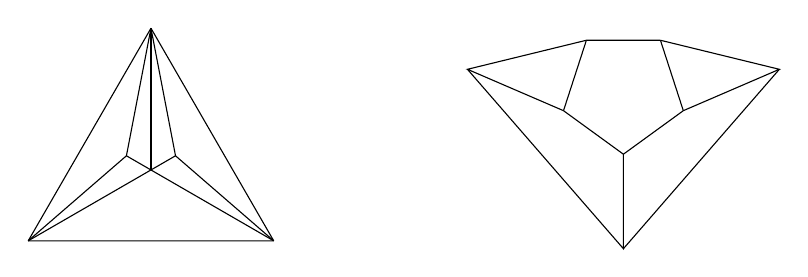
\begin{tikzpicture}[scale=1]

\begin{scope}[scale=0.9]
\foreach \x in {1,...,3}
{
\draw[rotate=120*\x]
  (90:2) -- (210:2);
\draw[rotate=120*\x]
  (90:2) -- (0:0);

 }
\draw (90:2) -- (150:0.4) -- (210:2);  
  \draw (0:0) -- (150:0.4);
\begin{scope}[xscale=-1]
 \draw (90:2) -- (150:0.4) -- (210:2);  
\draw (0:0) -- (150:0.4);  x
\end{scope}
\end{scope}

  
\begin{scope}[rotate=90,yshift=-6cm,xscale=-1,xshift=-1cm]

\foreach \x in {1,...,5}
{
\draw[rotate=72*\x]
	(0:0.8) -- (72:0.8);
}



 \draw (0:.8) --(0:2) -- (98:2);
 \draw (262:2) -- (0:2);
 \draw (216:.8) --(262:2) -- (288:.8);
 \draw (72:.8) --(98:2) -- (144:.8);
\end{scope}

 \end{tikzpicture}
 
\caption{$PCnC_{12}$ and the dual.}
\label{PCnC12}
\end{figure}

\begin{figure}[htp]
\centering
 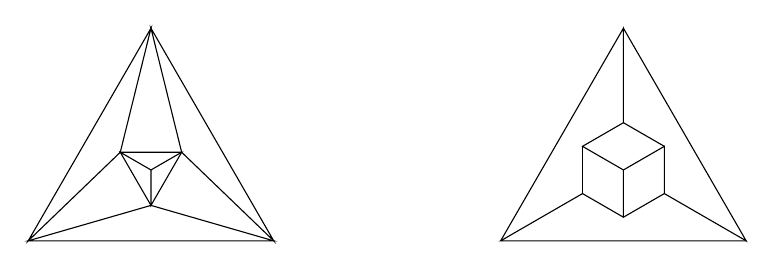
\begin{tikzpicture}[scale=1]

\begin{scope}[scale=0.9]
\foreach \x in {1,...,3}
{
\draw[rotate=120*\x]
  (90:2) -- (210:2)--(150:0.5)--cycle;
\draw[rotate=120*\x]
  (0:0) --  (150:0.5) -- (270:0.5);
 }
\end{scope}

  
\begin{scope}[scale=0.6,xshift=10cm]
\foreach \x in {0,...,2}
{
\draw[rotate=120*\x]  (210:3)--(90:3) -- (90:1) -- (150:1)--(0:0);
 \draw[rotate=120*\x] (210:1)--(150:1);
}
\end{scope}
 \end{tikzpicture}
\caption{$PCnC_{15}$ and the dual.}
\label{PCnC15}
\end{figure}


\begin{figure}[htp]
\centering
 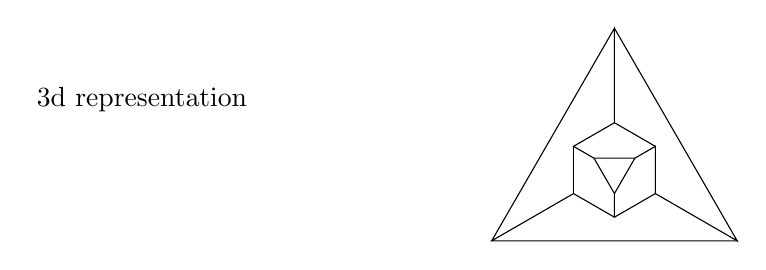
\begin{tikzpicture}[scale=1]

\begin{scope}[scale=0.9]
\node at (0,1)
{3d representation};
\end{scope}

  
\begin{scope}[scale=0.6,xshift=10cm]
\foreach \x in {0,...,2}
{
\draw[rotate=120*\x]  (210:3)--(90:3) -- (90:1) -- (150:1)--(150:.5)--(30:.5);
 \draw[rotate=120*\x] (210:1)--(150:1);
}
\end{scope}
 \end{tikzpicture}
\caption{$PCnC_{18_1}$~$(J_{84})$ and the dual.}
\label{PCnC181}
\end{figure}
\begin{figure}[htp]
\centering
 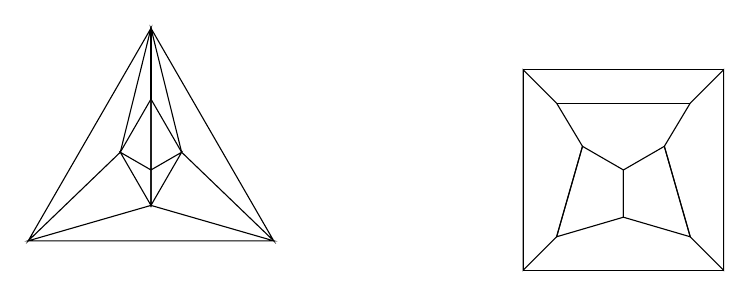
\begin{tikzpicture}[scale=1]

\begin{scope}[scale=0.9]
\foreach \x in {1,...,3}
{
\draw[rotate=120*\x]
  (90:2) -- (210:2)--(150:0.5)--cycle;
}

 % \draw[rotate=120*\x]  (0:0) --  (150:0.5) -- (270:0.5);
 \draw  (0:0) --  (150:0.5) -- (270:0.5)--(90:1);
 \draw  (0:0) --  (30:0.5) -- (270:0.5)--(90:1);

 \draw (30:.5) -- (90:1) -- (150:.5);
 \draw (90:2) -- (90:1);
\end{scope}

  
\begin{scope}[scale=0.6,xshift=10cm]
\draw  (135:3)--(135:2) -- (150:1) -- (225:2)--(225:3)--cycle;
 \draw (0:0)--(150:1)--(225:2)--(270:1)--cycle;
 \draw (45:2)--(135:2);
 \draw (45:3)--(135:3);
 \draw (225:3)--(315:3);  
\end{scope}
\begin{scope}[scale=0.6,xshift=10cm,xscale=-1]
\draw  (135:3)--(135:2) -- (150:1) -- (225:2)--(225:3)--cycle;
 \draw (0:0)--(150:1)--(225:2)--(270:1)--cycle;
 \draw (45:2)--(135:2);
 \draw (45:3)--(135:3);
 \draw (225:3)--(315:3);  
\end{scope}

 \end{tikzpicture}
\caption{$PCnC_{18_2}$ and the dual.}
\label{PCnC182}
\end{figure}



\begin{figure}[htp]
\centering
 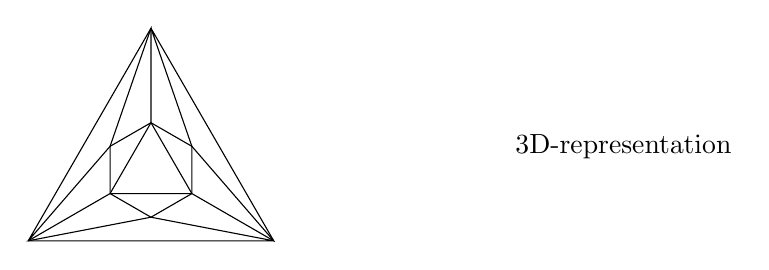
\begin{tikzpicture}[scale=1]
\begin{scope}[scale=0.6,yshift=1.5cm]
\foreach \x in {0,...,2}
{
\draw[rotate=120*\x]  (210:3)--(90:3) -- (90:1) -- (150:1)--cycle;
 \draw[rotate=120*\x] (210:1)--(150:1)--(90:3);
  \draw[rotate=120*\x] (-150:1)--(90:1);
}
\end{scope}



\begin{scope}[scale=0.6,xshift=10cm]
%\foreach \x in {1,...,3}
%{
%\draw[rotate=120*\x]  (90:2) -- (210:2)--(150:0.5)--cycle;
%\draw[rotate=120*\x]
% (0:0) --  (150:0.5) -- (270:0.5);
 % }
 \node at (0,2) {3D-representation};
\end{scope}

 \end{tikzpicture}
\caption{$PCnC_{21}$ $(J_{51})$ and the dual.}
\label{PCnC21}
\end{figure} 

\begin{figure}[htp]
\centering
 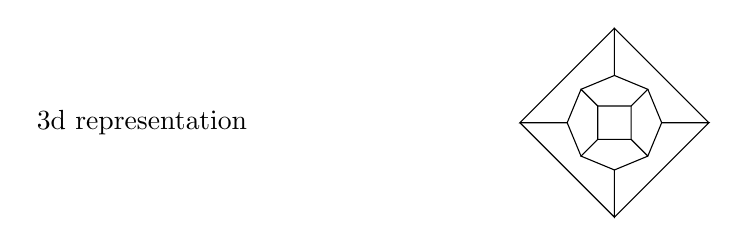
\begin{tikzpicture}[scale=1]

\begin{scope}[scale=0.9]
\node at (0,1)
{3d representation};
\end{scope}

  
  
\begin{scope}[scale=0.6,xshift=10cm,yshift=1.5cm,yscale=-1]
\foreach \x in {0,...,3}
{
\draw[rotate=90*\x]  (180:2)--(90:2) -- (90:1) -- (135:1)--(135:.5)--(45:.5);
 \draw[rotate=90*\x] (180:1)--(135:1);
}
\end{scope}
 \end{tikzpicture}
\caption{$PCnC_{24}$~$(J_{17})$ and the dual.}
\label{PCnC24}
\end{figure}


\begin{figure}[htp]
\centering
 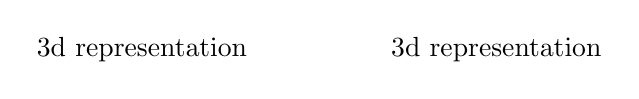
\begin{tikzpicture}[scale=1]

\begin{scope}[scale=0.9]
\node at (0,1)
{3d representation};
\end{scope}

\begin{scope}[scale=0.9,xshift=5cm]
\node at (0,1)
{3d representation};
\end{scope}

\end{tikzpicture}
\caption{$PCnC_{30}$~(Regular icosahedron) and the dual.}
\label{PCnC30}
\end{figure}
